\documentclass{tufte-handout}
\usepackage[utf8]{inputenc}
\usepackage[T1]{fontenc}
\usepackage{tikz}
\usepackage{listings}

\title{Head First Java: Chapter 9 Notes}
\lstset{language=java, basicstyle={\small\ttfamily}, breaklines=true}

\begin{document}

    \maketitle

    \section*{Memory Management in Java, the Stack, and the Heap}
    The stack and the heap are concepts that aid in understanding on how Java allocate memory to various entities in written programs. 

    \begin{itemize}
        \item Stack --- The stack can be visualized as a literal stack of frames. Each frame is an invoked method within a class. Methods and variables can be thought of ``living'' on a stack. Consider:

        \begin{lstlisting}
public void method1() {
    String x = ``Doing stuff '';
    System.out.println(x);
    method2(x);
} 

public void method2(String y) {
    String z = y + ``again '';
    System.out.println(z);
    method3();
}

public void method3  {
    String s = ``Nope I am done'';
    System.out.println(s);
}
        \end{lstlisting}

        Above is a series of methods that calls each other. When compiled and ran, the stack will initially look like this:
        \begin{center}
            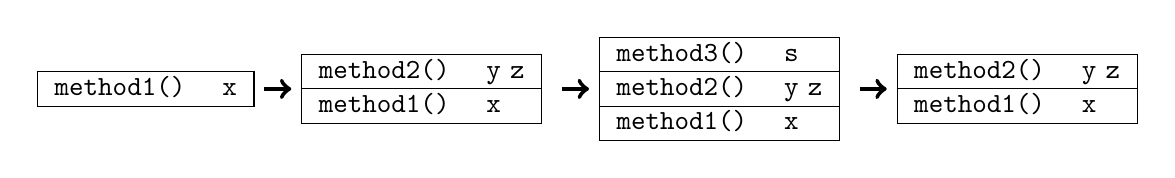
\begin{tikzpicture}
                \node (a) {
                    \begin{tabular}{ |l| }
                        \hline \texttt{\textbf{method1()}} \quad \texttt{x} \\ 
                        \hline     
                    \end{tabular}
                };
                \node[xshift=2cm] (b) at (a.east) {
                    \begin{tabular}{ |l| }
                        \hline \texttt{\textbf{method2()}} \quad \texttt{y} \texttt{z} \\ 
                        \hline \texttt{\textbf{method1()}} \quad \texttt{x} \\  
                        \hline     
                    \end{tabular}
                };
                \node (c) at (b.east) {};
                \draw[->,ultra thick](a)--(b);
                \node[xshift=2cm] (d) at (c.east) {
                    \begin{tabular}{ |l| }
                        \hline \texttt{\textbf{method3()}} \quad \texttt{s} \\ 
                        \hline \texttt{\textbf{method2()}} \quad \texttt{y} \texttt{z} \\  
                        \hline \texttt{\textbf{method1()}} \quad \texttt{x} \\
                        \hline    
                    \end{tabular}
                };
                \draw[->,ultra thick](c)--(d);
                \node (e) at (d.east) {};
                \node[xshift=2cm] (f) at (e.east) {
                    \begin{tabular}{ |l| }
                        \hline \texttt{\textbf{method2()}} \quad \texttt{y} \texttt{z} \\ 
                        \hline \texttt{\textbf{method1()}} \quad \texttt{x} \\  
                        \hline    
                    \end{tabular}
                };
                \draw[->,ultra thick](e)--(f);
            \end{tikzpicture}
        \end{center}

        Based on the code, \texttt{method1()} was invoked first; it is the first frame in the stack. Within this stack, the \emph{local variable} \texttt{x} is created by \texttt{method1} and ``lives'' in its frame on the stack. Because the \texttt{method1()} frame is at the top of the stack at this moment, \texttt{method1()} and its associated local variables (\texttt{x} in this case) is said to be \emph{in scope} and therefore accessible. Next, \texttt{method1()} calls \texttt{method2()} within its own code. Another frame containing \texttt{method2()} and its local variables (\texttt{y} and \texttt{z}) is not added to the top of the stack. Because only the frame at the \emph{top} of the stack is in scope, only the \texttt{method2()} frame and everything in it is in scope and thus accessible from the rest of the program. While not in scope, \texttt{method1()} and its variables cannot be accessed, but it is still ``alive'' (\textit{i.e.} it still exist in memory.) Within \texttt{method2()}, \texttt{method(3)} was called, and thus it is pushed to the top of the stack along with its local variable \texttt{s}. At this point, both \texttt{method2()} and \texttt{method1()} are no longer in scope and their variables are unavailable. Because \texttt{method3()} does not call any other methods itself, it completes its task (in this case, printing ``Nope I am done'' to the screen) and its frame along with its variables are ``popped'' off the stack. Once off the stack, all variables within that frame is ``dead'' and is permanently inaccessible. This stack continues to run with the \texttt{method2()} frame in scope now, and so forth. All local variables, regardless if they are primitive or object references, exist in the stack and behave the same way. In the case of object reference variables, the actual object being references do not exist in the stack, however, they exist in the heap.

        \item Heap --- Java objects (not object references) exist in the memory heap. The heap is unlike the stack as they are not ordered and scopes has no meaning here. Recall object creation and object reference declaration in Java is a three step process:

        \begin{enumerate}
            \item \texttt{\textbf{Object o} = new Object} --- declaration of a new \texttt{Object} class object reference variable in the stack or the heap.
            \item \texttt{Object o = \textbf{new Object}} --- instantiation of a new \texttt{Object} class object in the heap.
            \item \texttt{Object o \textbf{=} new Object} --- connecting the object reference variable \texttt{o} either on the stack or in the heap to the actual object in the heap. 
        \end{enumerate}

        While this is only one line of code in Java, three different things are occurring. If the object reference variable is a local variable of a method, then it exists in the frame of its creating method on the stack. However, if the object reference variable is an instance variable, then it exist in the heap. In either case, whatever object the object reference variable is referencing exists in the heap. Note that often object reference instance variable can be declared without assigning and instantiating an object (not possible with local variables), in this case the object reference variable still remains in the heap awaiting assignment. 

        An important note can be observed here: object reference variables can be declared without assigning them to an object (existing or newly instantiated), but objects \textbf{CANNOT} be instantiated without assigning them to an object reference variable. The implication here is that if the object reference variable assigned to an object ceased to exist in memory, the assigned object essentially also ease to exist (in reality, the object remains in the heap, but it is no longer accessible and is marked for \emph{garbage collection}.)

        \end{itemize}

    \section*{Object Creation and Constructors}
    Objects are instantiated in Java by constructors. Explicitly writing constructor code within a class is optional as if they are unwritten the compiler will write one itself. When the \texttt{new} keyword is used during object reference variable declaration and object assignment/instantiation, the constructor is called (whether it is explicitly written code or implicitly written by the compiler.) Consider the class \texttt{Duck}:

    \begin{lstlisting}
public class Duck {
    public Duck() {             // Constructor code begins here
        System.out.println(``Quack'');
    }
}
    \end{lstlisting}

    The above code differs from the generic constructor code that the compiling would write if unwritten only with the \texttt{System.out.println(``Quack'')} line. By writing this \texttt{public Duck()\{\}} constructor code in the class, the compiling will no longer write the generic constructor into the bytecode but will run the explicitly written constructor instead. In this case, every time a \texttt{Duck} object is instantiated, the constructor will also print \texttt{``Quack''} to the screen.

    Written explicit constructors into a class is useful especially when external information is needed (either from the user or from elsewhere in the program) for the instantiation of the object. Consider the following modified \texttt{Duck} class:

    \begin{lstlisting}
public class Duck {
    private int size;       // Instance variable
    public Duck() {         // Constructor
        System.out.println(size);
    }
    public void setSize(int newSize) { // Setter method
        size = newSize;
    }
}
    \end{lstlisting}

    The danger here is that a new \texttt{Duck} object can be instantiated by \texttt{Duck aDuck = new Duck();} without any problems, but the user or the rest of the program will have to immediately run the \texttt{aDuck.setSize()} method, otherwise the \texttt{Duck} object will not have a size, which can cause unexpected behavior for the rest of the program. One way to avoid this is to assign a default value to the instance variable \texttt{size} (\textit{e.g.} \texttt{private int size = 42;}), but due to encapsulation this is not enough if flexibility is needed for users to set there own \texttt{size} value. In this case, multiple constructors should be coded by \emph{overloading}:

    \begin{lstlisting}
public class Duck {
    private int size;       
    public Duck() {
        this(42);         
    }
    public Duck(int userSize) {
        size = userSize;
        System.out.println(size); 
    }
}
    \end{lstlisting}

    When a new \texttt{Duck} object is instantiated, one or the other constructor above will be called depending if an appropriate argument is passed or not. In this case, if an \texttt{int} argument was passed, a new \texttt{Duck} object is instantiated with the user supplied size, which is also printed on the screen. If no argument was passed, then the constructor with the \texttt{this()} method is called. The \texttt{this()} helps with consistency if multiple constructor is needed; it will called the most appropriate constructor for the current object depending on the argument passed to \texttt{this()}. In this case, \texttt{this(42);} passed a valid \texttt{int} argument for the \texttt{public Duck(int userSize) \{\}} constructor, therefore it acts like a default if the user or the rest of the program instantiated a new \texttt{Duck} object without supplying an argument, and assigning \texttt{42} to \texttt{size}. If \texttt{this()} is to be used in a constructor, it \textbf{must} be the first line of the code.

    In summary:

    \begin{enumerate}
        \item A constructor is the code that runs when a new object is instantiated (\textit{e.g.} the \texttt{new} keyword was used).
        \item A constructor must have the same name as the class it is written in, but have no return type.
        \item A constructor is implicitly written by the compiler if not explicitly written in the class.
        \item Constructors can be \emph{overloaded}, meaning multiple constructors can be written for the same class. However, the overloaded constructors must have different argument lists (argument orders, types, etc.)
    \end{enumerate}

    \section*{Constructors and Inheritance}
    Constructors exist in all classes, whether or not they are a superclass, a subclass, or both. Consider the following:

    \begin{lstlisting}
public class Animal {
    public Animal() {
        System.out.println(``Making an animal'')
    }
}

public class Hippo extends Animal {
    public Hippo() {
        System.out.println(``Making a Hippo'')
    }
} 
    \end{lstlisting}

    Constructors behaves like methods, and thus they exist on the stack. When a \texttt{Hippo} object is instantiated (by \texttt{Hippo h = new Hippo();} for example), the stack evolves:
        
    \begin{center}
        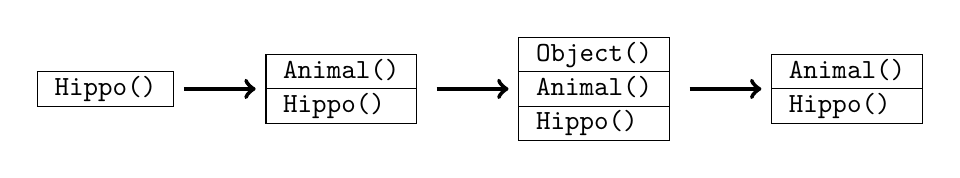
\begin{tikzpicture}
            \node (a) {
                \begin{tabular}{ |l| }
                    \hline \texttt{Hippo()} \\ 
                    \hline     
                \end{tabular}
            };
            \node[xshift=2cm] (b) at (a.east) {
                \begin{tabular}{ |l| }
                    \hline \texttt{Animal()} \\ 
                    \hline \texttt{Hippo()} \\  
                    \hline     
                \end{tabular}
            };
            \node (c) at (b.east) {};
            \draw[->,ultra thick](a)--(b);
            \node[xshift=2cm] (d) at (c.east) {
                \begin{tabular}{ |l| }
                    \hline \texttt{Object()} \\ 
                    \hline \texttt{Animal()} \\  
                    \hline \texttt{Hippo()} \\
                    \hline    
                \end{tabular}
            };
            \draw[->,ultra thick](c)--(d);
            \node (e) at (d.east) {};
            \node[xshift=2cm] (f) at (e.east) {
                \begin{tabular}{ |l| }
                    \hline \texttt{Animal()} \\ 
                    \hline \texttt{Hippo()} \\  
                    \hline    
                \end{tabular}
            };
            \draw[->,ultra thick](e)--(f);
        \end{tikzpicture}
    \end{center}

    The \texttt{Hippo()} constructor is first called, and remain on the top of the stack. However, \texttt{Hippo()} inherits from \texttt{Animal}, its superclass, and therefore before any code in \texttt{Hippo()} is ran, the constructor \texttt{Animal()} is pushed to the top of the stack, putting \texttt{Hippo()} and any of its code (and if exist, variables) out of scope and accessibility. Recall that all objects are ultimately subclasses of class \texttt{Object}, so its constructor \texttt{Object()} is pushed to the top of the stack. Any code in \texttt{Animal()} is not out of scope as well until \texttt{Object()} completes and is popped off the stack. Hence, the screen output when instantiating a \texttt{Hippo} object will first be ``\texttt{Making an Animal}'' then ``\texttt{Making a Hippo}''. 

    When a subclass object is instantiated, its superclass constructor is always called first, whether or not it is explicitly written out. The listing below is essentially the same from the one above:

    \begin{lstlisting}
public class Animal {
    public Animal() {
        super();
        System.out.println(``Making an animal'')
    }
}

public class Hippo extends Animal {
    public Hippo() {
        super();
        System.out.println(``Making a Hippo'')
    }
} 
    \end{lstlisting}

    The \texttt{super()} above is a call of the immediate superclass constructor. Therefore, the \texttt{super()} in \texttt{Hippo()} calls the \texttt{Animal()} constructor, and the \texttt{super()} in \texttt{Animal()} calls the \texttt{Object()} constructor. If \texttt{super()} is not explicitly stated in a constructor, the compiler will write it implicitly. If written implicitly by the compiler, \texttt{super()} is always called without any arguments.

    Arguments can be passed to \texttt{super()} if it is appropriate. If we modify the \texttt{Animal} and \texttt{Hippo} class:

    \begin{lstlisting}
public abstract class Animal {
    private String name;
    public String getName() {
        return name();
    }
    public Animal(String userName) {
        name = userName;
    }
}

public class Hippo extends Animal {
    public Hippo(String hippoName) {
        super(hippoName);
    }
} 
    \end{lstlisting}
    The \texttt{Animal} class is now flagged \texttt{abstract} and therefore cannot be instantiated. It also contains an encapsulated \texttt{String} variable \texttt{name} that is not assigned value, a getter method that returns \texttt{name}, and a constructor that requires a \texttt{String} argument \texttt{userName} that it assigns to \texttt{name}. \texttt{Hippo} is a subclass of \texttt{Animal}, its constructor is explicitly written to require \texttt{String} argument \texttt{hippoName}. Within the code body of \texttt{Hippo()}, \texttt{super()} is explicitly called and passing the argument \texttt{hippoName}. Because \texttt{Animal} is the immediate superclass of \texttt{Hippo}, when \texttt{super(hippoName)} was called, the \texttt{Animal()} constructor was called and \texttt{hippoName} is passed up the inheritance tree. When a \texttt{Hippo} object is instantiated with, for example, the \texttt{String} argument ``Buffy'', all constructors within the direct inheritance tree are called in the order of \texttt{Object()}, \texttt{Animal()}, and \texttt{Hippo}. An \texttt{Object} is instantiated first, then the \texttt{Animal} is instantiated and wrapped around the \texttt{Object} object, within it the instance variable \texttt{name}, to which ``Buffy'' is assigned its value, and finally the \texttt{Hippo} is instantiated wrapping around the \texttt{Animal}. 

    If the superclass has overloaded constructors (multiple constructors), when calling \texttt{super()} in its subclass' constructor the argument type and order will determine which superclass constructor is called. Consider:

    \begin{lstlisting}
public class Boo {
    public Boo(int i) {}
    public Boo(String s) {}
    public Boo(String s, int i) {}
}
    \end{lstlisting}

    The class \texttt{Boo} is overloaded with three constructors, each requiring different argument(s) type and order. If a subclass exist, it must include an explicit call to its superclass constructor, because a no-argument constructor for \texttt{Boo} was not provided. Calling \texttt{super()} in a subclass constructor will not compile. There are many possibilities here, for example, if \texttt{super(``boo'')} was used, then the \texttt{public Boo(String s) \{\}} constructor is called. If \texttt{super(42)} was used, then the \texttt{public Boo(int i) \{\}} is called, and so forth. 

    Note that if \texttt{super()} is to be used in a constructor, it \textbf{must} be the first line of code. Therefore, \texttt{this()} and \texttt{super()} cannot be used in the same constructor. 

    \section*{Garbage Collection}
    As mentioned previously, when objects in the heap ``dies'' or become permanently inaccessible in the memory, the JVM will automatically marked it as eligible for \emph{garbage collection}. This means that when JVM determines that more memory is needed, it will overwrite memories eligible for garbage collection that is no longer in need. Everything in Java occupies memory. Things that exist on the stack (methods, local variables, constructors, etc.) are marked for garbage collection once it is popped off the stack (note that being out of scope does not mean being marked for garbage collection, the inaccessibility is temporary in this case.) Instance variables exist in objects in the heap, and they are ``alive'' as long as the object they exist in are still alive (\textit{i.e.} NOT marked for garbage collection.) 

    Another way to look at this is that anything on the stack remains alive and accessible (if not now, then later), but once popped off the stack (the frame it resides in completes), it is marked for garbage collection and is gone forever. Things that are in the heap remains alive as long as a reference to it exist. Generally speaking, there are two main categories of things in Java that exists in the heap: Object reference variables, and objects themselves. Objects remain alive as long as there is some reference to it from the stack. Recall from previously that an object cannot be instantiated without assigning to a reference variable (\texttt{Object o = New Object()}). If that link is severed, then the object itself is marked for garbage collection and is gone forever. There are a number of ways this can occur:

    \begin{enumerate}
        \item The frame where the object reference variable resides in is popped off the stack. This occurs when a method (or a constructor etc.) completes its task. The object reference variable is marked for garbage collection and is gone forever, therefore the same is true to the object itself.
        \item The object reference variable is assigned to another object. Since an object reference variable can only be assigned to a single object at anytime, the original object no longer has a reference on the stack, and is marked for garbage collection.
        \item The object reference variable is set to \texttt{null}. This is the same case as above. Essentially Java tells the object reference variable to sever its link to the object. As above, the object itself is then marked for garbage collection.
    \end{enumerate}

    Object reference variables themselves is a more complicated case as they can both exist on the stack as local variables or within an object in the heap as instance variables (this is true to primitive variables as well). Object reference variables that exist on the stack obeys the same rules, once popped off the stack they are marked for garbage collection. In the heap, object reference variables do not exist on their own but are inside actual objects. In this case, these object reference variables in the heap exist as long as the objects they reside remains ``alive''. If those objects are marked for garbage collection, so do all instance variables that reside within. 


\end{document}